\documentclass[12pt]{article}
\usepackage{graphicx}
\usepackage{amsmath}
\usepackage{float}
\usepackage[english]{babel}
\usepackage[english = american]{csquotes}
\MakeOuterQuote{"}
\usepackage[pdfpagemode=useNone,pdfstartview=FitH,colorlinks=true,linkcolor=blue,citecolor=blue,urlcolor=blue]{hyperref}
\usepackage[all]{hypcap}

\title{Single-Variable Calculus}
\author{physicsnerd}
\begin{document}

\maketitle
\tableofcontents

\section{Overview}
Calculus is the study of change. 
There are two main branches to calculus: differential and integral calculus. 
Differential calculus studies the slopes of lines, or the rate of change, using the derivative. 
Integral calculus studies the area under a curve. 
Many problems in many fields of science boil down to one of these two problems. 
Here, we will go over how to solve problems in the main fields of calculus, some applications of calculus, and finally some next steps in your study of calculus.

\section{Terms to Know}

\begin{itemize}
\item Slope: slope is defined as rise over run, or, more simply, how "steep" a line is. 
If a line is going "down", it has negative slope; if it is going "up" it has positive slope.
\item Speed: the change in position over time. 
You might be going 70 miles per hour in your car. 
Well, your  position is changing by 70 miles, every hour.
\item Velocity: speed, but with direction. 
For example, you might be biking at a speed of 10 miles per hour, and heading north. 
That's a velocity.
\item Acceleration: the change in velocity or speed over time. 
You might accelerate by a mile per minute, starting from 70 miles per hour. 
After 30 minutes, you'll be going 100 miles per hour, and your
speed will still be increasing. At that point, it's a good idea to
decelerate, or have a negative change in velocity/speed, and hope a
police officer hasn't seen you.
\item Function: something that takes in a number and spits out another
number. We usually write a function as $f(x)$, or $x(m)$, or $g(x)$, or
h(x)...something along those lines. We then say that as "$f$ of $x$". It
just means what a function $f$ evaluates too when you plug in a number $x$.
\item 9.81 m/s: the terminal acceleration of an object. Basically,
let's say you drop an object. It can't accelerate any faster than that
speed, no matter what. Blame gravity.
\item Work: a physics concept (we're not talking about a job here).
Basically, let's say you pick up a book and bring it to the kitchen
table. You just exerted force on an object. You just did work. Note
that in physics, if you haven't moved anything, you haven't done any
work. Basically, the amount of work you've done depends on the force
you've exerted (which in turn depends on mass and acceleration) and
displacement (or how far you've moved an object from it's original
location).
\end{itemize}


\section{Limits}

\chapter{Intuition of Limits}
The purpose of limits is to find what a function approaches at a certain number that it is not defined for. 
For example, let's say we have the function $f(x) = \frac{x^2}{x}$ and $x = 0$ in this particular case. 
Since we are not allowed to divide by zero, this function is not defined there. 
However, the function may approach a certain number.

\begin{figure}[H]
\caption{Function approaching $1$ as $x$ goes to $0$}
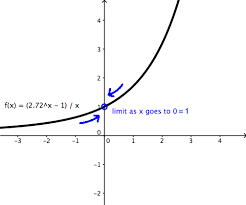
\includegraphics[scale=0.8]{../images.png}
\end{figure}

In the above graph, while the function is not defined at $0$, it approaches, or comes near to, $1$. 
There are several different "types" of limits and rules for calculating them. 
\chapter{Types of Limits}

The first type of limit you could call an "easy" limit. 
All you have to do is plug in the number you are approaching for your variable, because the function doesn't violate any rules like we described above. 
So for example, if you have the limit

\begin{equation*}
    \lim\limits_{x\rightarrow 1} x
\end{equation*}

You would just get 1. 
The second type of limit could be called a "$\frac{0}{0}$" limit. 
It does violate the rules, and we have to do some algebraic manipulation to get it into a form we can work with. 
This might be done via factoring a polynomial, normalizing the denominator or numerator, or some such method.

A quick algebra side-note here on how to do these things. 
Factoring a polynomial mainly references factoring quadratics, or equations of the form $ax^2 + bx + c$ ($=0$). 
We factor the left side by using this general method: find the factors of $ac$ and see which add up to $b$. 
Note that you can change the signs of the factors, that is, if you have $ac = 10$ and the factors are $1, \, 2, \, 5, \, 10$, and $b = 3$, you can do $5-2 = 3$. 
After this, we then take those two numbers, $5$ and $-2$ and rewrite it as $ax^2 + 5x -2x + c$. 
We then put parentheses in: $(ax^2 + 5x) + (-2x + c)$. 
Finally, we factor out the biggest common number (or variable) out of each of the parentheses.

Let's do this with a real problem. 
\begin{equation*}
    x^2 - x - 12
\end{equation*}
For $ac$, we get $1\times -12$, or $-12$. 
For $b$, we get $-1$. 
The factors of $12$ are $1, \, 2, \, 3, \, 4, \, 6, \, 12$. $-4\times 3 = -12$ and $-4+3 = -1$. 
So now we write 
\begin{equation*}
    x^2 - 4x + 3x - 12
\end{equation*}
Now, we put in the parentheses and get
\begin{equation*}
    (x^2-4x)+(3x-12)
\end{equation*}
Now for the last step, factoring. 
For the first parenthesis, we can take out $x$, and in the second parenthesis, we can take out $3$, so we get
\begin{equation*}
    x(x-4)+3(x-4)
\end{equation*}
Note that if the two parenthesis' contents are not the same, then you have done something wrong. 
Now, we can rewrite this expression as 
\begin{equation*}
    (x+3)(x-4)
\end{equation*}
The equation is now factored.

The other thing of note here is rationalizing the denominator or numerator. 
Normally, we rationalize the denominator to get a radical out of the denominator, but we can also do this for the numerator. 
To do this, we multiply by expression on the numerator or the denominator over itself. 
Let's say we have the expression $\frac{\sqrt{x}}{1}$. 
Then we would multiply by $\frac{\sqrt{x}}{\sqrt{x}}$ and simplify. 
Note that if instead we had an expression like $\frac{\sqrt{x}+1}{1}$ we would multiply by $\frac{\sqrt{x}-1}{\sqrt{x}-1}$. 
We switched the sign on the $1$ from $+$ to $-$. This is called taking the "conjugate" of the expression.

With these tools in hand, we can now start solving the second type of limit. 
Let us take as an example 
\begin{equation*}
    \lim\limits_{x\rightarrow -3}\frac{x^2-x-12}{x+3}
\end{equation*}
We can clearly see that if we just plug it in, there will be a zero in the denominator. 
Instead, we can try employing an algebraic tool. 
You might recognize the quadratic on the top as the one we factored earlier. 
Let us then replace that expression with its factored form:
\begin{equation*}
    \lim\limits_{x\rightarrow -3}\frac{(x+3)(x-4)}{x+3}
\end{equation*}
Now, we can cancel the $x+3$ on the top and bottom of the fraction. 
This then leaves us with
\begin{equation*}
    \lim\limits_{x\rightarrow -3}x-4
\end{equation*}
The limit is now one of our "easy" limits, so we can simply plug in $-3$. The answer is $-7$.

Now we have our final type of limit, the "$\frac{\text{not zero}}{0}$" limit. 
This type of limit is a bit different from the other two types of limits. 
It requires a bit more intuition. As an example, let's say we are trying to solve the problem
\begin{equation*}
    \lim\limits_{x\rightarrow 0}\frac{1}{x}
\end{equation*}
To solve this, we must first solve
\begin{equation*}
    \lim\limits_{x\rightarrow 0^+}\frac{1}{x}
\end{equation*}
and
\begin{equation*}
    \lim\limits_{x\rightarrow 0^-}\frac{1}{x}
\end{equation*}
First, let's examine the second problem. 
The $+$ sign means it is a right limit - that is, we are approaching zero from the left. 
What does that mean? Well, let's say we have a number line like the one below.

\begin{figure}[H]
\caption{Approaching zero}
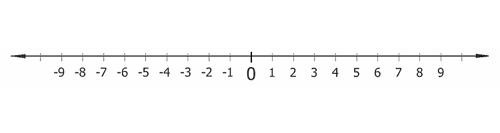
\includegraphics[scale=0.75]{../numberline.jpg}
\end{figure}

To approach from the right means that $x$ will be represented by tiny positive numbers, like $0.00001$ and $0.0000001$. 
They will get closer and closer to $0$. 
So, what does this mean? 
It means the answer to this particular limit will be whatever $\frac{1}{\text{really small positive number}}$ is. 
So let's take some examples. 
If we have $\frac{1}{0.00001}$ we get $100000$. 
If we have something closer to zero, like $\frac{1}{0.0000001}$ we get $10000000$. 
In other words, we are approaching infinity.
So the answer to this limit, approached from the right, is $+\infty$, or just $\infty$. 
Now, let's do the next one. 
This time, we are approaching zero from the left. Now we are dividing by small negative numbers. Try a few on a calculator and see what you get!

It turns out that this approaches $-\infty$. 
So the answer to the third limit in that list we started with is $-\infty$. 
Now, to solve the first limit. 
If we take the second two limits and their answer is the same, the first limit has a solution: the answer to the second two limits! 
However, the second two limits had different solutions. That means the answer to the first limit is undefined.


\section{Problems}
\begin{enumerate}
    \item $$\lim\limits_{x\rightarrow 3} 2x+5$$
    \item $$\lim\limits_{x\rightarrow 4} \frac{x^2-16}{x-4}$$
    \item $$\lim\limits_{x\rightarrow 9} \frac{\sqrt{x}-3}{x-9}$$
    \item $$\lim\limits_{x\rightarrow 0} \frac{1}{x^2}$$
    \item $$\lim\limits_{x\rightarrow 1} \frac{\sqrt{x}-1}{x-1}$$
\end{enumerate}

\section{Differential}

\subsection{Intuition Behind Derivatives}
Differential calculus is all about finding the slope of a curve. 
First, let's consider a normal case, finding the slope of a straight line. 
We take in two points, and find the change in x and change in y ($\Delta x$ and $\Delta y$). 
This can be written as $\frac{\Delta y}{\Delta x}$ or $\frac{\text{rise}}{\text{run}}$.

\begin{figure}[H]
\caption{Average Slope}
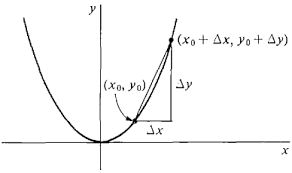
\includegraphics[scale=1]{../download.png}
\end{figure}

The above diagram illustrates this process on a curve. 
We pick two points on the line and find the average slope. 
However, this process is clearly not very accurate. 
Imagine that we move the two points closer and closer together. 
The closer they are, the more accurate the slope is for that small section of line, until eventually we make it so that there is only one point. 
That is, we are finding instantaneous slope, or the slope at one point of the line.

The derivative does that for the whole line, taking in a function and giving a new function that represents the slope. 
For example, let's say we shoot a cannonball.

\begin{figure}[H]
\caption{Trajectory of cannonball}
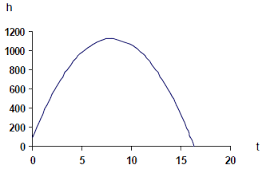
\includegraphics[scale=1]{../imgres.png}
\end{figure}

Here, the y-axis represents the height of the cannonball in meters and the x-axis indicates time in seconds. 
Notice that at the beginning the slope is positive, until eventually the graph reaches its peak and the slope is zero, and then the graph starts going down and the slope becomes negative. 
The derivative of this graph would then look something like this:

\begin{figure}[H]
\caption{Derivative of trajectory of cannonball}
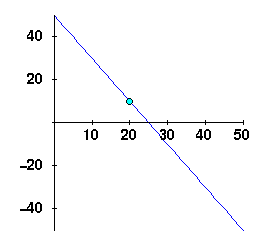
\includegraphics[scale=0.8]{../derivative.png}
\end{figure}

This is what is happening "behind the scenes" when we calculate derivatives.
However, it is important to note that, going back to the example of the cannonball, where the cannonball started does not affect the slope. 
If the whole graph is shifted up or down, the slope stays the same (as long as the proportions are kept the same). 
This, it turns out, is why we need to add the $c$ in a indefinite integral. 
\subsection{Derivatives and Integrals}
Derivatives and integrals are inverses of each other. 
That is, they undo each other, like division undoes multiplication and subtraction undoes addition. 
(This is called the "fundamental theorem of calculus".)
So, because when going from an integral back to a derivative there is some uncertainty which graph you are looking at (parallel lines, for instance, have the same slope, but they have different "heights"), you have to add the $c$ when solving an indefinite integral.
\subsection{Basic Derivative Rules}
Below is a table with some solutions to various derivatives. Note that $c$ is a constant and $n$ is non-zero. Note that the $'$ symbol is pronounced prime, and is another way to write that we are taking the derivative. 


\begin{tabular}{c|c}
    $f(x)$ & $\frac{df}{dx} = f'$\\
    \hline
       $7$  & $0$ \\
        $c$ & $0$ \\
        $x$ & $1$ \\
        $cx$ & $c$ \\
        $x^2$ & $2x$ \\
        $cx^2$ & $2cx$ \\
        $x^3$ & $3x^2$ \\
        $x^n$ & $nx^{n-1}$ \\
        $\sin x$ & $\cos x$ \\
        $\cos x$ & $-\sin x$ \\
        $- \sin x$ & $- \cos x$ \\
        $-\cos x$ & $\sin x$
\end{tabular}

Like integrals, derivatives are distributive over addition.
There are some interesting rules that make working with derivatives easier: the product rule, the quotient rule, and the chain rule. 

Let's start with the chain rule. 
If we have a function within a function in a derivative, like $\sin(\cos(x))$, we can assign a name to each function, like $g(x) = \cos(x)$ and $h(x) = \sin(x)$, and then follow this simple rule: $h'(g(x)) \cdot g'(x)$. 
So what does this mean? 
Well, let's plug it in. 
Plugging this in gives $\sin'(\cos(x)) \cdot \cos'(x)$. 
So the derivative of $\sin$ is $\cos$, so we write $\cos(\cos(x))$ for the first part, and the derivative of $\cos$ is $-\sin$, so we write $-\sin(x)$ for the second part. 
So now we have $\cos(\cos(x)) \cdot -\sin(x)$. 
This is the derivative of our original function.

Now, let's examine the product rule. 
If we have two functions, $u(x)$ and $v(x)$, and we want to take the derivative of $u\cdot v$, then we can do $u \cdot \frac{dv}{dx}+ v\cdot\frac{du}{dx}$. 
In other words, we multiply the first function by the derivative of the second function and then add the second function times the derivative of the first. 
For example, if we have $\sin(x)\cdot\cos(x)$ we would do $u(x) = \sin(x)$ and $v(x) = \cos(x)$. 
Then we would plug it in to our formula: $\sin(x)\cdot\frac{d}{dx}\cos(x) + \cos(x)\cdot\frac{d}{dx}\sin(x)$ which simplifies to $\sin\cdot -\sin(x) + \cos(x)\cdot\cos(x)$ or $-\sin^2(x)+\cos^2(x)$, which is our derivative of the original function.

Finally, the quotient rule. 
If we have two functions, $g(x)$ and $h(x)$, and we wish to take the derivative of $\frac{g(x)}{h(x)}$, we can follow the rule $\frac{g'(x)h(x)-h'(x)g(x)}{[h(x)]^2}$. 
While this may look rather complicated, it really isn't too bad. 
Let's use the example of $g(x) = \sin(x)$ and $h(x) = \cos(x)$. 
We plug it all in to get $\frac{\sin'(x)\cdot\cos(x) -\cos'(x)\cdot\sin(x)}{\cos^2(x)}$
which simplifies to $\frac{\cos(x)\cdot\cos(x)--\sin(x)\cdot\sin(x)}{\cos^2(x)} = \frac{\cos^2(x)+sin^2(x)}{\cos^2(x)} = \sin^2(x)$. 
So therefore, $\sin^2(x)$ is our derivative.
\subsection{Formal Definition of a Derivative}
Now, let's say you forget these rules, or come across something you can't use these rules on. In this case, you can use the formal definition of a derivative. When looking at this definition, remember that $\Delta$ means "change in" whatever variable comes afterwards (i.e., $\Delta x$ means the change in x). Given a function $f(t)$, the derivative of $f(t)$ ($\frac{df(t)}{dt}$) is \begin{equation}
    \lim\limits_{\Delta t\rightarrow 0}\frac{\Delta f}{\Delta t} = \lim\limits_{\Delta t\rightarrow 0}\frac{f(t+\Delta t)-f(t)}{\Delta t}
\end{equation}
Let's try using this on a derivative - say, the derivative of $f(t)$ where $f(t) = t^2$. We have to solve $\lim\limits_{\Delta t\rightarrow 0}\frac{f(t+\Delta t)-f(t)}{\Delta t}$. Remember that the rule is that the input to $f$ must be squared, so for the first term, we need to square $t+\Delta t$ - $(t+\Delta t)(t+\Delta t) = t^2+t\Delta t+t\Delta t + \Delta t^2 = t^2+2t\Delta t+\Delta t^2$. That's the first term on top of the fraction. The second term is just $f(t)$ - which we've been told equals $t^2$. Since we subtract this from the first term, the two cancel, leaving $\frac{2t\Delta t+\Delta t^2}{\Delta t}$. We then divide, getting $2t+\Delta t$. Now we have to apply the limit in front. Remember that if there will be no mathematically impossible results, we can just plug in the limit - i.e., in this case, $2t+0$ or just $2t$, which is our result. We can of course check this using our earlier exponent rule (which we can actually derive; see exercise six and solution), and $2t$ is still the result.


\section{Problems}
\begin{enumerate}
    \item $5x$
    \item $6x^3 - 9x + 4$
    \item $2t^4 - 13t$
    \item $x^{-1}$
    \item $\sqrt{x}$
\end{enumerate}

\section{Integral}

\chapter{Intuition Behind the Integral}
The point of the integral is to find the area under a curve. 
One of the interesting applications of integration is finding the displacement of an object - the displacement corresponds to an object's trajectory; that is, the area under a graph of velocity versus time is displacement.

While we don't actually need to do the following, this is generally what is happening. 

\begin{centering}
\begin{figure}[H]
\caption{Riemann Sum}
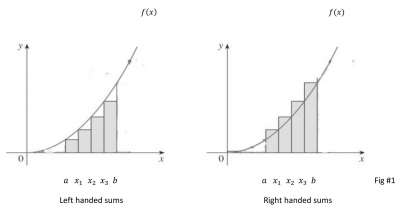
\includegraphics[scale=0.8]{../rieman.jpg}
\end{figure}
\end{centering}

Basically, we pick a specified width, let's say $w$. 
Then, we create several rectangles, with a width $w$ and a height that is just under the curve we are trying to find the area of. 
Then, we do this again, but this time the height is just above the curve. 
We take the average of the two numbers, and get the area of the curve. 
The smaller we make $w$, the more accurate the number, and at width $0$, we basically have lines, which fit the curve perfectly. 
This is the point of an integral.
\chapter{Basic Integration Rules}
Below is a table of some of the basic outputs of integrals. Some of these will make more sense after going through derivatives.

\begin{tabular}{l|l}
    $f(x)$ & $\int f(x) \, dx$\\
    \hline
     $0$ & $0+c$ \\
     $1$ & $x+c$ \\
     $D$ & $Dx+c$ \\
     $2x$ & $x^2 + c$ \\
     $x$ & $x^2/2 + c$ \\
     $x^2$ & $x^3/3 + c$ \\
     $x^n$ & $x^{n+1}/n+1 + c$
\end{tabular}

In these, $c$ and $D$ are constants and $x$ is some variable.

Note that after every integral, we must put $dx$ or $dt$ or $d$ and then whatever variable we are using in our integral. 
The second important thing to note is that these results have $c$ after them because they are ``indefinite'' integrals - that is, because we don't have a specific bound on the integral, we must add a constant $c$ to show that there is some range in what the answers will be. 
This is again something that will make more sense after going over derivatives.

So there are indefinite integrals, but there are also "definite" integrals. 
We write them as $\int^b_a$. Basically, let's say we have the integral $\int x \, dx$. 
We integrate the inside according to the table, getting $x^2/2$, but instead of adding the constant $c$, we then plug in $b$ and $a$ in for $x$ as follows: 
\begin{equation*}
    (b^2/2) - (a^2/2)
\end{equation*}

This gives our answer, and we do not need to put in $c$.

There is another important thing about integrals. For an integral such as $\int x+x \, dx$, we can change this into

\begin{equation*}
    \int x \, dx + \int x \, dx
\end{equation*}

That is, integrals are a linear function, much like multiplication ($5*(5+2)$ can be rewritten $5*5 + 5*2$) and many other functions. We can also factor out constants; for example, given $\int 2x + 3x \, dx$, we can change this into 

\begin{equation*}
    2\cdot \int x \, dx + 3 \cdot \int x \, dx
\end{equation*}

Also remember that you can simplify within a problem; i.e., given $x(x^2 + x^3)$ you can then multiply and get $x^3 + x^4$. 
Finally, there is a helpful rule for integrals - the product rule. 
If you have a function $v(x)$ and a function $u(x)$, and you wish to find the derivative of $u(x)\cdot v(x)$, you can follow the rule $u\cdot v - \int v\frac{du}{dx}\, dx$.
\chapter{Derivatives and Integrals}
Derivatives and integrals are inverses of each other. 
That is, they undo each other, like division undoes multiplication and subtraction undoes addition. 
(This is called the "fundamental theorem of calculus".)
So, because when going from an integral back to a derivative there is some uncertainty which graph you are looking at (parallel lines, for instance, have the same slope, but they have different "heights"), you have to add the $c$ when solving an indefinite integral. 
\chapter{Formal Definition of an Integral}
\section{Summations}
A summation is a simple method of notation that shortens long repetitive addition operations. Let's look at an example:

\begin{equation}
\sum\limits_{n=0}^{n=5} 2n
\end{equation}

Here, the expression $n=0$ under the summation symbol means that to start the sum, we plug in $0$ for $n$. The expression $n=5$ on top means we continue until we have plugged in $5$ for $n$. Expanded, this summation means

\begin{equation}
2\times 0+2\times 1+2\times 2+2\times 3+2\times 4+2\times 5
\end{equation}

which means the answer is $30$. Think back to the section on the intuition behind integrals for why we need this. We're really summing up a bunch of small rectangles. 
\section{Formal definition of indefinite integrals}
\section{Formal definition of definite integrals}

\section{Problems}
Solve the following integrals:

\begin{enumerate}
    \item $\int x \, dx$
    \item $\int x^2-5 \, dx$
    \item $\int^5_0 x^2 \, dx$
    \item $\int^5_3 x^2 \, dx$
    \item $\int^5_3 x^2 + 1 \, dx$
\end{enumerate}

\section{Applications}

\subsection{Applicable Fields}
Now we get to the most interesting part of calculus: its applications. 
Here, we are going to focus on only a few applications, but there are many applications of calculus, across many fields, such as economics, sociology, physics, mathematics itself, chemistry, astronomy, and others. 
Calculus is key in many fields.
\subsection{Physics Applications}
The main application we are going to look at is work, as defined by physics. 
Interestingly, there is an integral definition of work - that is, work can be defined using an integral.

\begin{equation*}
    \int^b_a f(x) \, dx
\end{equation*}

What does this mean? 
Well, first, $f(x)$ is a function representing force, where $x$ is displacement, which, as Newton's second law states, is $F = ma$ - that is, force is mass times acceleration. 
Second, $b - a$ should equal the displacement, or how much the object is moved. This is because $b$ and $a$ are what we are substituting for $x$, which is displacement.
This is easier to illustrate with a few problems.

For example, let's say we have a bowling ball, rolled with a force equal to the function $f(x) = 2x+3$ (where the resulting number is in Newtons). 
We want to find out how much work it takes to roll it from the start of our lane down to the end of the lane, 10 meters away.

Well, here, this is easy. All we do is plug in the numbers into our formula for work! 

\begin{equation*}
    \int^{10}_0 2x+3 \, dx
\end{equation*}

Remember that $a$ and $b$ together represent displacement. 
We're rolling the bowling ball from the start, $0$, to the end of the lane, $10$ meters away. 
So that represents $a$ and $b$ respectively. 
The force, $f(x)$, is simple to plug in. 
So now, we follow the rules for integrating. 
In this case, we get $2\frac{x^2}{2}+3x\mid^{10}_0$. 
Note that this last part, the line with the superscripts, is just a bit of notation, saying that we plug in $10$ and $0$ and subtract according to the rules of definite integrals. 
It just allows us to integrate and write that down. 

So now that we have this, we plug it in as we would for normal definite integrals, and so we get $(2\cdot\frac{10^2}{2}+3\cdot 10) - (2\cdot\frac{0^2}{2}+3\cdot 0)$ and then we simplify. 
The whole second half comes to zero, so we now have $2\cdot\frac{10^2}{2}+3\cdot 10$. 
Then, we have $2\cdot \frac{100}{2}+ 30$ or $2\cdot 50 + 30$ or $130$. 
Now we look at units. 
We have meters and newtons, so now when we multiply those two, we have joules (a unit of work). 
So our answer is $130$ joules. 
Note that it is very important to keep track of your units. If you don't know a unit of force, work, or distance, look it up! Think logically.

A quick note on Hooke's Law: when considering the work required to stretch a spring, you can assume that the force ($f(x)$) needed to stretch a spring a distance $x$ beyond its natural length is proportional to $x$. 
In other words, we have $f(x) = cx$ where $x$ is the distance the spring is stretched and $c$ is some constant.
\subsection{Economics Applications (?)}

\subsection{Problems}
For the second problem, the spring can be assumed to obey Hooke's Law.

\begin{enumerate}
    \item If throwing a baseball requires a force equivalent to $f(x) = 5x^2$ pounds then find the work necessary to throw a baseball from third to first base (about $127$ feet).
    \item If a ten-pound force stretches an elastic spring one inch, how much work is done in stretching the spring one foot?
\end{enumerate}

\section{What Next?}

What we've been looking at here is called single variable calculus - which, clearly enough, involves integrals and derivatives with only one variable. 
However, there is such a thing as multivariable calculus, adding more variables, and even more usefulness to an already incredibly useful tool. 
This is a good next thing to study after single-variable calculus. 
There is also a form of calculus called vector calculus (to study this, it is a good idea to know
linear algebra) which is useful to know. 
Finally, there is the field of differential equations, from simpler, "ordinary" differential equations to more complex partial differential equations. 
All of these fields are incredibly interesting and well worth studying.


\medskip

\section{Worked Solutions}

A few of the problems have been taken from Apostol's Calculus, Volume 1.

\section*{Limits}
\begin{enumerate}
\item \begin{equation*}
    \lim\limits_{x\rightarrow 3} 2x+5 = 2(3)+5 = 11
\end{equation*} This is just the "easy" type of limit.
\item \begin{equation*}
    \lim\limits_{x\rightarrow 4}\frac{x^2-16}{x-4} = \lim\limits_{x\rightarrow 4}\frac{(x-4)(x+4)}{x-4} = \lim\limits_{x\rightarrow 4}x+4 = 8
\end{equation*} Here we have to do some algebraic manipulation - factoring. Then, after we cancel, it converts to the easy form, and we can just plug in $x$ and go.
\item \begin{align*}
    & \lim\limits_{x\rightarrow 9}\frac{\sqrt{x}-3}{x-9}=  \lim\limits_{x\rightarrow 9}\left(\frac{\sqrt{x}-3}{x-9}\right) \left(\frac{\sqrt{x}+3}{\sqrt{x+3}}\right) = \\  &\lim\limits_{x\rightarrow 9} \frac{x+3\sqrt{x}-3\sqrt{x}-9}{(x-9) (\sqrt{x}+3)}=\lim\limits_{x\rightarrow 9}\frac{x-9}{(x-9)(\sqrt{x}+3)} = \\ & \lim\limits_{x\rightarrow 9}\frac{1}{\sqrt{x}+3} =\frac{1}{\sqrt{9}+3}=\frac{1}{6}
\end{align*}
Here, again, we must do some algebraic manipulation. 
We rationalize the denominator by multiplying by the conjugate over itself (we must do that, so if we divide it equals one) and then the top and bottom cancel, and so we are left with something we can simply plug in. 
Don't be tricked here - this did not convert into a "$\frac{1}{0}$" limit so we don't need to do anything special.
\item \begin{align*}
    &\lim\limits_{x\rightarrow 0} \frac{1}{x^2}\\
    &\lim\limits_{x\rightarrow 0^+} \frac{1}{x^2} = +\infty\\
    &\lim\limits_{x\rightarrow 0^-} \frac{1}{x^2} = +\infty\\
    &\lim\limits_{x\rightarrow 0} \frac{1}{x^2} = +\infty
\end{align*}
Remember how for $\frac{1}{0}$ limits we must do the right and left limit, and check if their result is equal. 
To do that, we look at approaching $0$ first from the right (so very small positive numbers) and then square them, making them even smaller, and then we divide one by these tiny numbers, giving a huger and huger output as we approach zero. 
Therefore, this gives positive infinity. 
Now, when approaching from the left, you might expect negative infinity to be the answer, but we are squaring $x$, meaning that this turns into tiny positive numbers, so again, we are left with positive infinity.
\item \begin{equation*}
    \lim\limits_{x\rightarrow 1} \frac{\sqrt{x}-1}{x-1} = \lim\limits_{x\rightarrow 1} \frac{\sqrt{x}-1}{x-1} \cdot \frac{\sqrt{x}+1}{\sqrt{x}+1} = \lim\limits_{x\rightarrow 1} \frac{x-1}{(x-1)(\sqrt{x}+1)}=\lim\limits_{x\rightarrow 1} \frac{1}{\sqrt{x}+1} = \frac{1}{2}
\end{equation*}
Here we are rationalizing the numerator again. Again, don't be tricked - it does not turn into a $\frac{1}{0}$ limit.
\end{enumerate}

\section*{Integrals} 
\begin{enumerate}
\item $\int x \, dx = \frac{x^2}{2}+c$ For this one, all you have to do is use the table given. 
Because it is an indefinite integral, don't forget to add $c$!
\item $\int x^2 - 5 \,dx = \int x^2 \, dx - \int 5 \, dx = \frac{x^3}{3}-5x + c$ Remember that the integral is distributive over addition and subtraction. 
Also, remember that there is only one $c$ added to the solution of any indefinite integral.
\item $\int^5_0 x^2 \, dx = \frac{x^3}{3}\mid^5_0 = \frac{5^3}{3}-\frac{0^3}{3}=\frac{5^3}{3}=\frac{125}{3}$ Remember that $\mid^5_0$ is simply a piece of notation that allows us to keep track of what we are integrating over as we integrate.
\item $\int^5_0 x^2 \, dx = \frac{x^3}{3}\mid^5_0 = \frac{5^3}{3}-\frac{3^3}{3} = \frac{125}{3} - \frac{27}{3} = \frac{125}{3}-9$ Note that in this case (and the previous problem) you could simplify a bit further, but this is as far as we'll go.
\item $\int^5_3 x^2 + 1\, dx = \int^5_3 x^2 \, dx + \int^5_3 1 \, dx = \frac{x^3}{3}+x\mid^5_3 = \frac{5^3}{3}+5 - \frac{3^3}{3}+3 = \frac{125}{3}+5 - \frac{27}{3}+3 = \frac{125}{3}+5 - 12 = \frac{125}{3}-7$
\end{enumerate}

\section*{Derivatives}
\begin{enumerate}
\item $\frac{d}{dx} \, 5x = 5$ Here, we simply follow the rules in the table.
\item $\frac{d}{dx} \, 6x^2 - 9x + 4 = 12x - 9$ Remember that constants simply disappear, and the exponent rules outlined in the table.
\item $\frac{d}{dx} \, 2t^4 - 13t = 8t^3 - 13$
\item $\frac{d}{dx}\, x^{-1} = -x^{-2}$ 
\item $\frac{d}{dx}\, \sqrt{x} = \frac{d}{dx}\, x^{\frac{1}{2}} = \frac{1}{2}x^{-\frac{1}{2}}$ This one requires knowing how roots translate into exponents, but after that, it isn't so bad.
\item Our function is $f(t) = t^n$, so we plug this in and carry on. We have $\lim\limits_{\Delta t\rightarrow 0}\frac{(t+\Delta t)^n-t^n}{\Delta t}$. Here we can use the binomial theorem (this problem is a real challenge, so don't feel bad if you felt absolutely stuck here) which basically says that $(a+b)^n = a^n+na^{n-1}b+\frac{n(n-1)}{2}a^{n-2}b^2+\frac{n(n-1)(n-2)}{3}a^{n-3}b^3+...+b^n$. For our purposes, we only need the first two terms, because all the others shrink to zero due to the limit (you can check this yourself with a few examples) so you get $\lim\limits_{\Delta t\rightarrow 0}\frac{t^n+nt^{n-1}\Delta t-t^n}{\Delta t}=\lim\limits_{\Delta t\rightarrow 0}\frac{nt^{n-1}\Delta t}{\Delta t}=\lim\limits_{\Delta t\rightarrow 0}nt^{n-1}$ and here you'll notice that the limit doesn't apply anywhere, so you just have $nt^{n-1}$ - which is of course the exponent rule.
\end{enumerate}

\section*{Applications}
\begin{enumerate}
\item $f(x) = 5x^2 \; W = \int^b_a f(x) \, dx \; \int^127_0 5x^2 \, dx = 5\cdot \frac{x^3}{3}\mid^{127}_0 = \frac{127^3}{3}-\frac{0^3}{3} = \frac{127^3}{3} = \frac{2048383}{3} \,\text{foot-pounds}$
Remember here that $W$, or work, is equivalent to the integral $\int^b_a f(x) \, dx$. From there, we just plug in the force equation and go.
\item First, remember that according to Hooke's Law, force is proportional to $x$. 
So here we get $f(x) = 10x$. 
Then, we consider displacement - well, we're stretching the spring one foot, so $b=12$ and $a = 0$. 
Remember here that we're using inches! 
Now we plug it in: $\int^{12}_0 10x \, dx = 10\cdot\frac{x^2}{2}\mid^{12}_0$. 
Now we know that the second part will all come out to zero, so we are left with $10\cdot\frac{12^2}{2}$ or $10\cdot\frac{144}{2} = 10\cdot 72 = 720$ - but what are our units? 
Well, we are multiplying inches by pounds, so inch-pounds. 
But we can simplify to foot-pounds by dividing our answer by $12$. This gives us $60$ foot-pounds.
\end{enumerate}


\nocite{bluebrown}
\nocite{khanacademy}
\nocite{passcalculus}
\nocite{mitocw}
\nocite{paulmath}
\nocite{apostoli}
\nocite{apostolii}
\nocite{spivak}
\nocite{cartoon}


\bibliographystyle{plain}
\bibliography{resources}

\end{document}

